\chapter{OLS model inference and evaluation}
So now we know how to get slopes and the intercept. Now we need to get a handle on whether we can conclude anything substantive about them. There are two aspects to model evaluation: hypothesis tests of coefficients and evaluating model fit. These topics are of course connected and we see that when we test blocks of coefficients.

Let us consider, again, a model where wages are a function of education and other variables. In Tables~\ref{tab:wagesum} and~\ref{tab:wagereg} I referenced a dataset of 200 observations with three variables: hourly wages ("wage"), years of education ("edu"), and age. Table~\ref{tab:wagereg_all} displays three different models. The first model is simply
\begin{equation}
\hat{y}_i=\beta_0+\beta_1edu_i
\end{equation}
the second model adds age to the model
\begin{equation}
\hat{y}_i=\beta_0+\beta_1edu_i+\beta_2age_i
\end{equation}
and the final model adds a dichotomous female indicator
\begin{equation}
\hat{y}_i=\beta_0+\beta_1edu_i+\beta_2age_i+\beta_3female_i
\end{equation}
\begin{table}[htbp]\centering
 \caption{Models predicting wages
\label{tab:wagereg_all}}
\begin{tabular}{lccc}
\hline
Coefficients  &   Model 1  &   Model 2  &   Model 3  \\ \hline
edu     &    0.835***&    0.882***&    0.847***\\
      &   (0.195)  &   (0.184)  &   (0.184)  \\
age     &        &    0.218***&    0.229***\\
      &        &   (0.043)  &   (0.044)  \\
female   &        &        &   -2.033  \\
      &        &        &   (1.074)  \\
intercept  &    4.780  &   -3.866  &   -2.817  \\
      &   (2.682)  &   (3.061)  &   (3.091)  \\
\hline
\multicolumn{4}{l}{Model Statistics} \\
\hline
$N$   &   200.000  &   200.000  &   200.000  \\
$F$    &   18.410  &   22.947  &   16.692  \\
$R^2$   &    0.085  &    0.189  &    0.204  \\
$df$ Regression    &    1.000  &    2.000  &    3.000  \\
Sum of Squares Regression  &  1172.179  &  2603.472  &  2804.011  \\
$df$ Error    &   198.000  &   197.000  &   196.000  \\
Sum of Squares Error   &  12606.570  &  11175.277  &  10974.738  \\
\hline
\multicolumn{4}{l}{$SE$s in parentheses, $***p<0.001$} \\
\hline
\end{tabular}
\end{table}
Table~\ref{tab:wagereg_all} gives a lot information. First we get the slopes and intercept on the upper table. Second, we get model fit statistics on the lower table. In this section, I describe these measures.
\section{The variance and covariance of regression coefficients}
\label{sec:matrixv}
In statistics, we are obsessed with the variance of our estimators. The variance of the an estimator is the just the square of the standard error. Thus, once we know the variance of the estimator, we can just get the square root and use that for hypothesis testing. In matrix notation, the variance of the regression slopes is
\begin{equation}
\bf V\left({\hat{b}}\right)=\left(\frac{1}{N}X'X\right)^{-1}\sigma^2
\end{equation}
where $\sigma^2$ is the variance of the regression residuals, or
\begin{equation}
\sigma^2 = \frac{\sum_{i=1}^N\left(e_i-\bar{e}\right)^2}{N-p}
\end{equation}
and $\bf X'X$ is the sum of squares of the matrix of predictors. We can express this with conventional algebra in the bivariate regression model as
\begin{equation}\label{eq:olsb1var}
\mbox{var}\left(\beta_1\right)=\frac{\sigma^2}{\sum_{i=1}^N\left(x_i-\bar{x}\right)^2}
\end{equation}
and we can express the standard error of the slope as the square root of this
\begin{equation}
SE\left(\beta_1\right)=\sqrt{\frac{\sigma^2}{\sum_{i=1}^N\left(x_i-\bar{x}\right)^2}}
\end{equation}
Here we see that the variance, and thus the standard error, is a function of the variance in the residuals and the variance in the predictor. It's the variance in the predictor that is the big player here. The larger the variance in $x$, or the more $x$ is "spread out," the smaller the standard error.
This is related to this is the variance of predicted point, $\hat{y}_0$, where again the crucial ingredient is the variance of $x$
\begin{equation}\label{eq:varfit}
\mbox{var}\left(\hat{y}_0\right)=\left(\frac{\sigma^2}{N}+\frac{\left(x_0-\bar{x}\right)^2\sigma^2}{\sum_{i=1}^N\left(x_i-\bar{x}\right)^2}\right)\sigma^2
\end{equation}
Here, $\hat{y}_0$ is the predicted value of $y$ associated with a hypothetical value of $x$, $x_0$. We see that as the hypothetical value of $x$ moves away from the mean of $x$, that the variance will increase.  This formula allows us to construct a confidence interval for each prediction
\begin{equation}
CI\left(\hat{y}_0,\left(1-\alpha\right)\times100\right)=\hat{y}_0\pm t_{df,\alpha/2}\sqrt{\left(\frac{\sigma^2}{N}+\frac{\left(x_0-\bar{x}\right)^2\sigma^2}{\sum_{i=1}^N\left(x_i-\bar{x}\right)^2}\right)\sigma^2}
\end{equation}
Thus, the greater the variance in $x$, the smaller the confidence interval in any predicted value of $y$. A smaller confidence interval means that the range of possible slopes for $y$ is smaller.
\begin{figure}
   \centering
   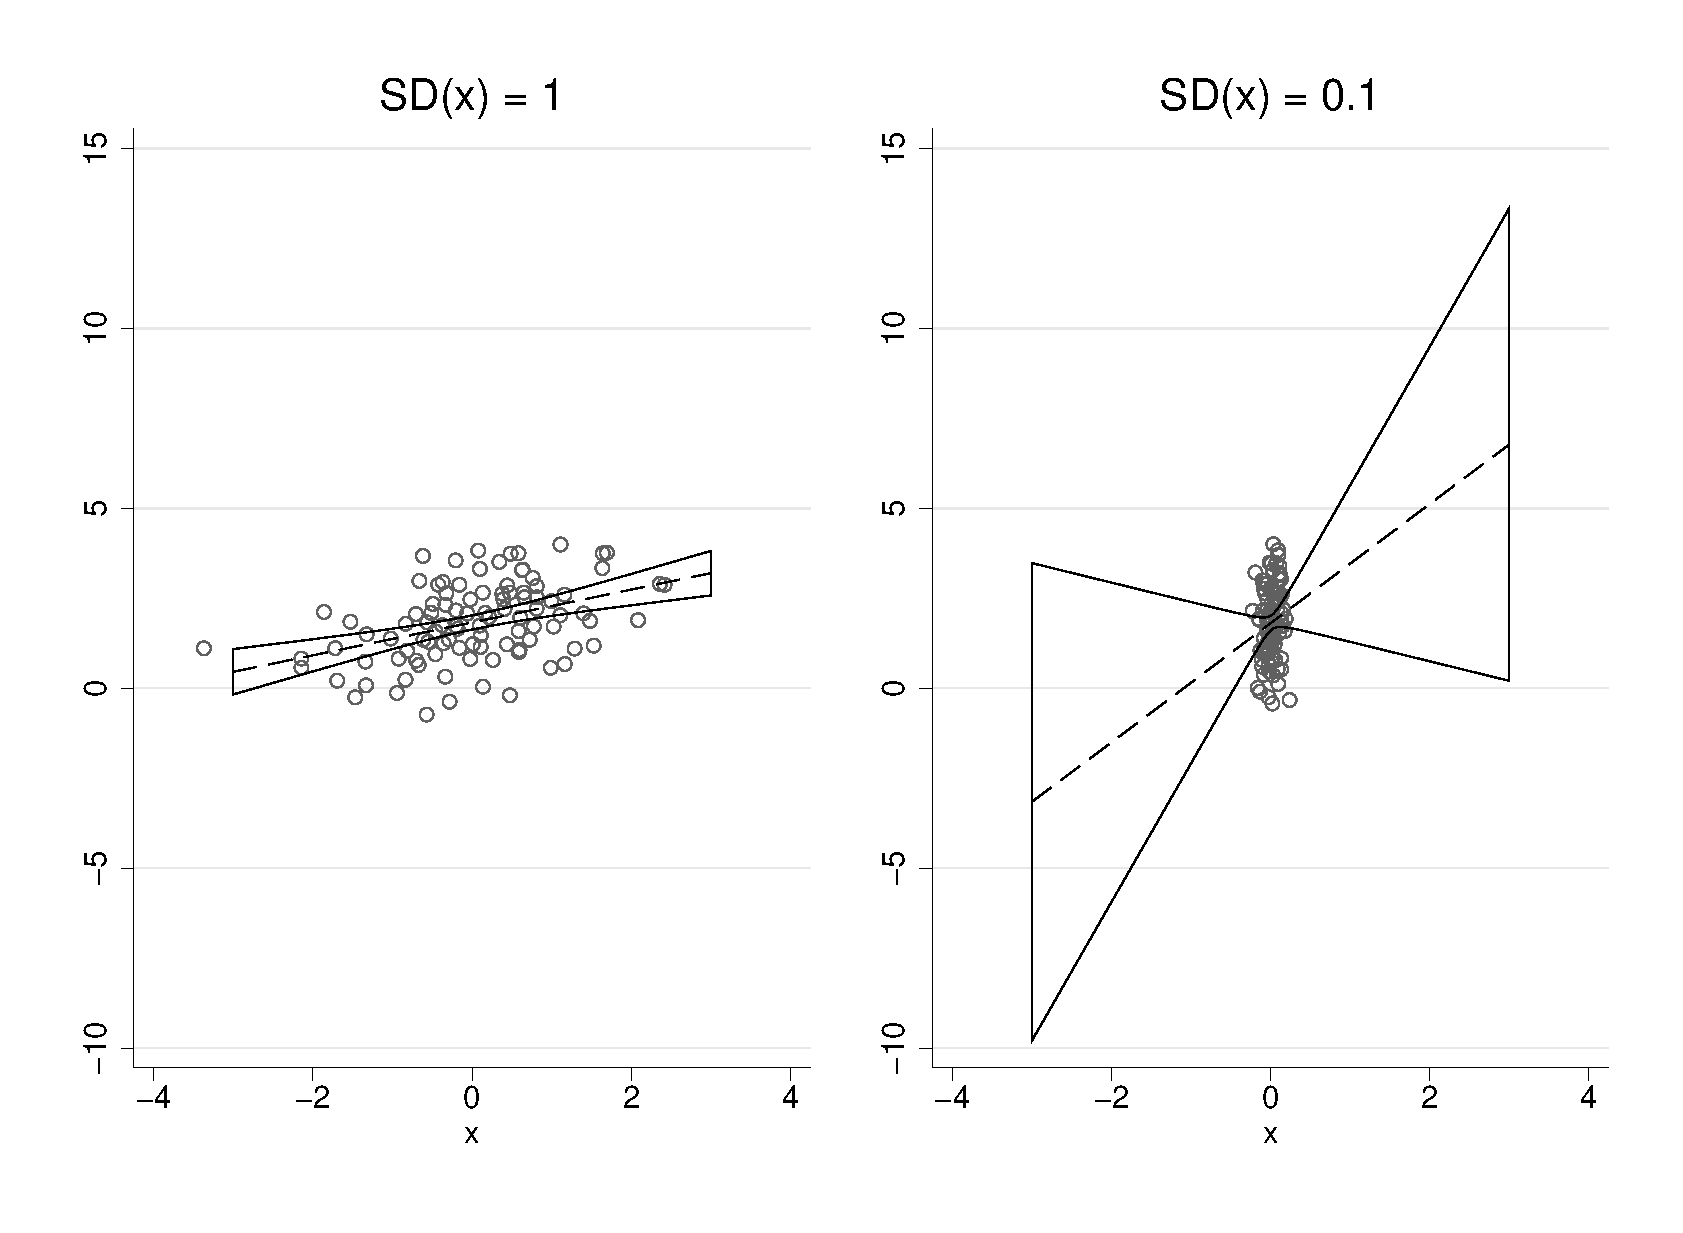
\includegraphics[angle=0,
           width=.75\textwidth]{cislope.eps}
   \caption{Variance of regression slopes as a function of the variance of $x$}
  \label{fig:cislopes}
\end{figure}
Figure~\ref{fig:cislopes} features this difference. The panel on the left is a situation in which $x$ has the larger standard deviation. We see that the slope is accurate and the 95 percent confidence interval (the fan like shape around the prediction line) of the prediction is pretty tight, implying a small standard error of the slope. The panel on the right, however, $x$ has a small standard deviation and we see that the range of possible slopes is large because the 95 percent confidence interval of values is quite high.
\section{Hypothesis testing with regression slopes}
Recall our hypothesis testing for the difference between means. We were testing the difference between two mean values of $y$, $\bar{y}_A$ and $\bar{y}_B$. Testing regression slopes is quite similar. Here we are testing the difference between a predicted value of $y$ when $x$ is equal to some arbitrary value, $A$ and the predicted value of $y$ when that value of $x$ increases by a single unit to $B$. In other words, we are comparing $\hat{y}_A$ and $\hat{y}_B$.

Obviously, since regression slopes reflect the difference in the predicted value of $y$ reflected in a one unit change in $x$, our regression slope reflects this difference. Here the null hypothesis is that this slope is 0, or that there is no relationship
\begin{equation}
H_0:\beta_p = 0
\end{equation}
and the alternative hypothesis is that this slope is something other than 0
\begin{equation}
H_1:\beta_p \ne 0
\end{equation}
Note that I use the term $\beta_p$ here because this applies for any coefficient, including the intercept. With the null hypothesis equal to 0, the form of our $t$-test is the slope divided by the standard error; c.f.,~\eqref{eq:ttest}
\begin{equation}
t=\frac{\beta_p-0}{SE\left(\beta_p\right)}=\frac{\beta_p}{SE\left(\beta_p\right)}
\end{equation}
This $t$-test has $N-p-1$ degrees of freedom, where $p$ is the number of predictors and we subtract 1 for the intercept as well.
Returning to our education and wages example in Table~\ref{tab:wagereg_all} (Model 1), we see that for every year of education, the average wages increase by about 83.5 cents. The standard error of this estimate is 0.195. The $t$-test for this coefficient is
\[
t=\frac{0.835}{0.195}=4.28
\]

The $df$ Error in the table tells us our degrees of freedom for this test. Using a computer or table, we can find that the probability of finding this slope if the null hypothesis were true is 0.00003, far below the $\alpha = 0.05$ threshold. Therefore, we say the effect is statistically significant. Most computer programs will tell you this probability, known as a $p$-value. Thus, we think that the slope is significantly different from 0 and thus we make the conclusion that an effect of education on wages is plausible.

We also test whether the intercept is equal to 0:
\[
t=\frac{4.780}{2.682}=1.78
\]
In this case, since the $p$-value is 0.077, and we cannot reject the null hypothesis, and we have to conclude that if someone with 0 years of education, there wages are practically 0, which of course makes intuitive sense.

Finally, since the intercept and slope are jointly estimated, we also estimate a covariance of these parameters
\begin{equation}
\mbox{cov}\left(\beta_0,\beta_1\right)=\sigma^2\left(\frac{-\bar{x}}{\sum_{i=1}^N\left(x_i-\bar{x}\right)^2}\right)
\end{equation}
which is actually estimated, along with the variances of the slopes themselves, in a matrix form as
\begin{equation}\label{eq:olsmatrixvar}
\bf V\left(\hat{b}\right) = \sigma^2\left(X'X\right)^{-1}
\end{equation}
which in in this case is
\[
\bf V\left(\hat{b}\right) =
\begin{bmatrix}
\mbox{var}\left(\beta_{edu}\right) & \mbox{cov}\left(\beta_{edu},\beta_{intercept}\right) \\
\mbox{cov}\left(\beta_{intercept},\beta_{edu}\right) & \mbox{var}\left(\beta_{intercept}\right) \\
\end{bmatrix}
=
\begin{bmatrix}
0.038 & -0.510 \\
-0.510 & 7.193 \\
\end{bmatrix}
\]
Note that $\mbox{var}\left(\beta_{intercept}\right)$ is the square of the standard error for the intercept and that $\mbox{var}\left(\beta_{edu}\right)$ is the square of the standard error for the slope. This doesn't have an immediate use in bi-variate regression, but in multiple regression it is a useful quantity for accurate testing differences between coefficients of predictors with formulas like
\begin{equation}
t=\frac{\beta_p-\beta_q}{\sqrt{\mbox{var}\left(\beta_p\right)+\mbox{var}\left(\beta_q\right)-2\mbox{cov}\left(\beta_p,\beta_q\right)}}
\end{equation}
\section{Model fit by way of ANOVA}

Folks often ignore the ANOVA table in regression output because they do not know why it's there. Here is a cool fact for bivariate regression: if you square the t-test of the slope, you find that it is equal to the F-test in the output. Least squares regression and ANOVA are very much related. Recall how in ANOVA we consider how the total sum of squares is decomposed into the sum of squares between groups and the sum of squares within groups
\begin{equation}
SST=SSW+SSB
\end{equation}
or
\begin{equation}
\sum_{j=1}^k\sum_{i=1}^{n_j}\left(y_{ij}-\bar{y}\right)^2=\sum_{j=1}^k\sum_{i=1}^{n_j}\left(y_{ij}-\bar{y}_j\right)^2+\sum_{j=1}^kn_j\left(\bar{y}_j-\bar{y}\right)^2
\end{equation}
The analogue in regression is that instead of group means, $\bar{y}_j$, we have predicted values of $y$ for a given value of $x$, $\hat{y}$. Instead of the sum of squares within groups ($SSW$), we have the sum of squares error ($SSE$), which is how each case deviates from it's predicted value. Instead of the sub of squares between ($SSB$), we have the sum of squares regression ($SSR$), which is how the regression prediction deviates from the overall mean of $y$,
\begin{equation}
SST=SSE+SSR
\end{equation}
or
\begin{equation}
\sum_{i=1}^{N}\left(y_{i}-\bar{y}\right)^2=\sum_{i=1}^{N}\left(y_{i}-\hat{y}_i\right)^2+\sum_{i=1}^N\left(\hat{y}_i-\bar{y}\right)^2
\end{equation}
\begin{figure}
   \centering
   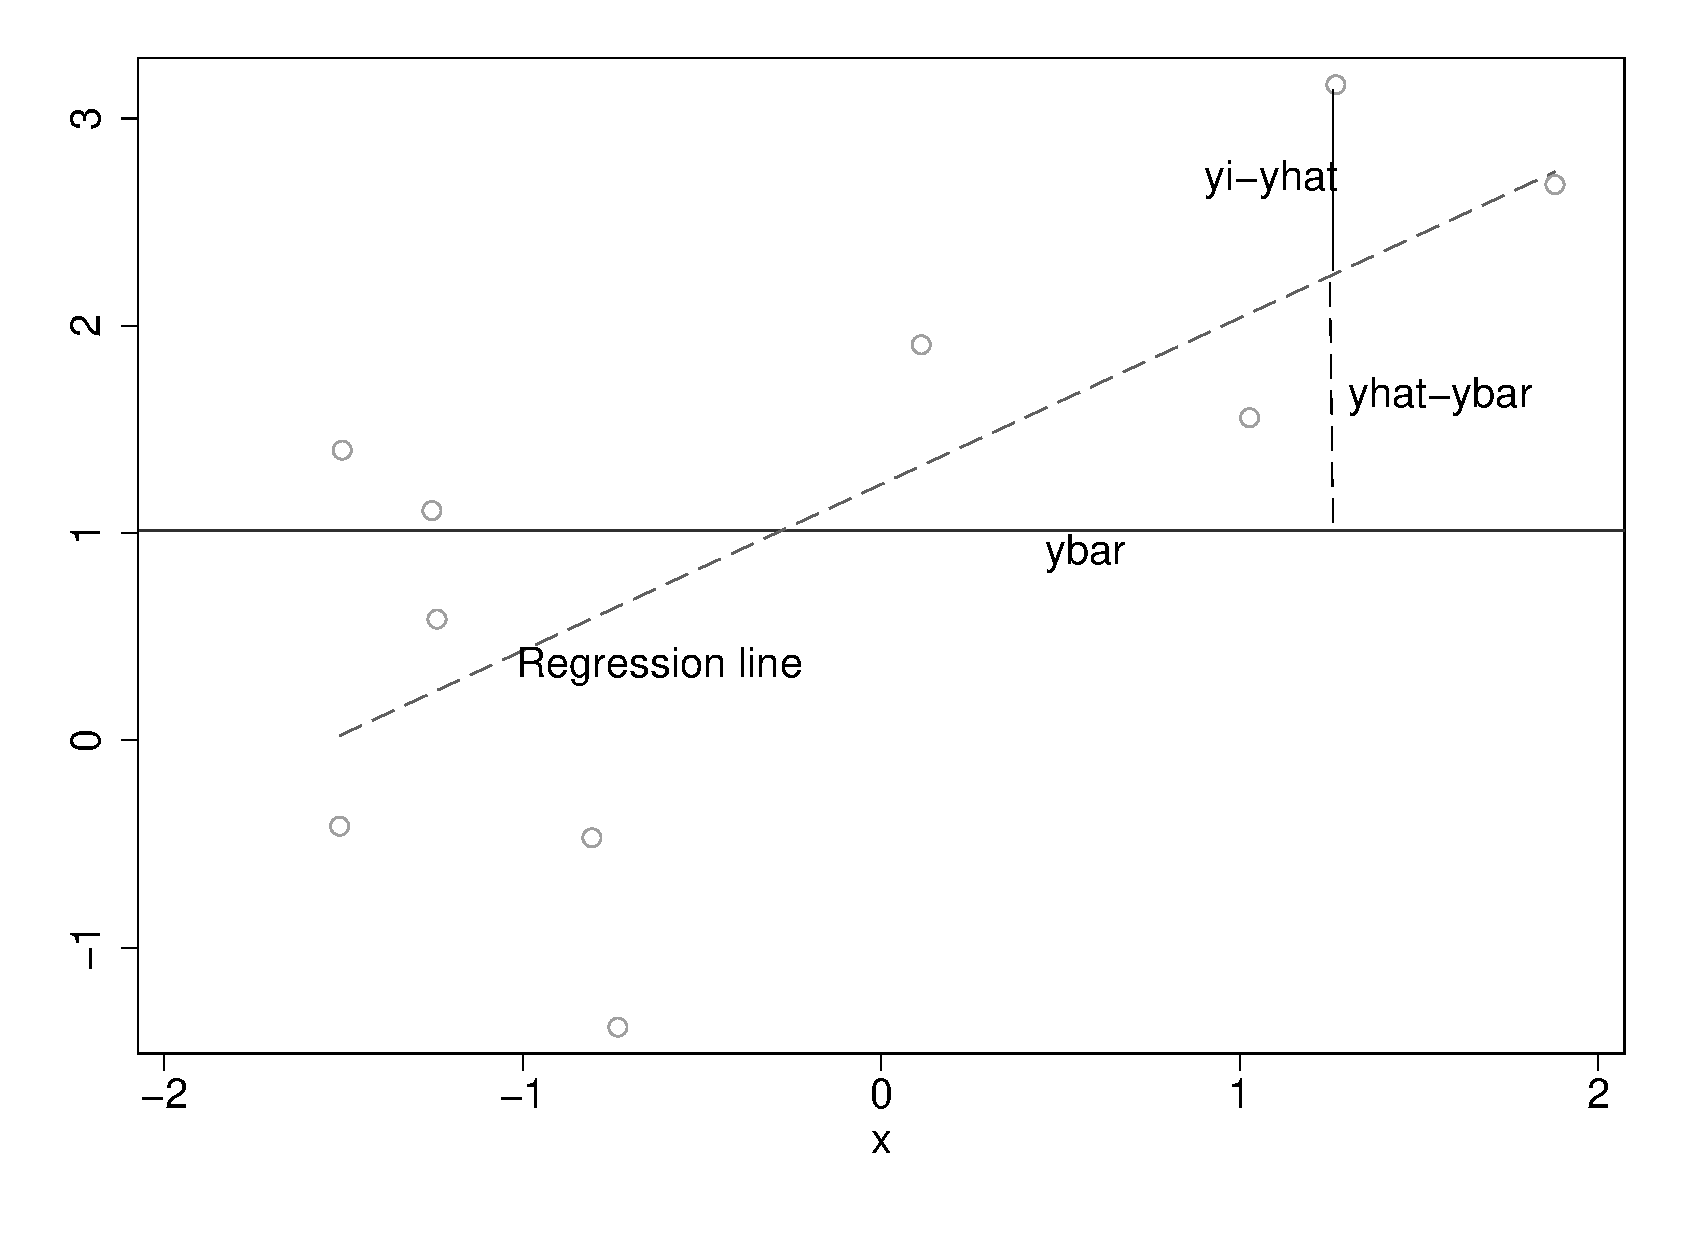
\includegraphics[angle=0,
           width=.75\textwidth]{anova.eps}
   \caption{The deviance of $y_i$ to $\hat{y}_i$ to $\bar{y}$}
  \label{fig:anova}
\end{figure}
This is visualized in Figure~\ref{fig:anova}, which is data from Table~\ref{tab:xy}. The solid line on the scatter plot is the overall mean of $y$, the dotted line with the slope is the regression fit line. We then take a single point and draw a solid vertical line from that point and the regression line. This represents $y_i-\hat{y}_i$. We then draw a dotted line from the predicted value of the regression line to the overall mean. This represents $\hat{y}_i-\bar{y}$ . The total difference between the observation and and the overall mean, $y_i-\bar{y}$, is the sum of these quantities.

With these quantities we can do an F-test to test whether the sum of squares residual is less than the sum of squares total
\begin{equation}
F=\frac{MSR}{MSE}
\end{equation}
where
\begin{equation}
MSR = \frac{SSR}{p}
\end{equation}
and
\begin{equation}
MSE = \frac{SSE}{N-p-1}
\end{equation}
This test is then evaluated against the F distribution with ($p, N-p-1$) degrees of freedom. The degrees of freedom for the sum of squares error is $N-p-1$, just like the $t$-test, and the degrees of freedom for the sum of squares regression is $p$, again where $p$ is the number of predictors excluding the intercept.

Examining the fit statistics from our wage and education example, Model 1 in Table~\ref{tab:wagereg_all}, the sum of squares from the model is 1,172.179 and the sum of squares error is 12,606.570. We then see the degrees of freedom ($df$) for each quantity. We can test the fit of the model with the $F$-test,
\[
F=\frac{\left(\frac{1172.179}{1}\right)}{\left(\frac{12606.570}{198}\right)}=18.410
\]
which is associated with a probability ($p$-value) of 0.00003. This should be familiar, that's because the unrounded $t$-test was 4.29, the square of which is 18.410. This means that our model contributes something to explaining the variation in wages.
\section{Model fit by way of $R^2$}
Another statistic reported in our regression output is $R^2$. Substantively, this is a measure of how much variation is "explained" in the data. The calculation for $R^2$ is simply the ratio of the sum of square regression to the sum of squares total ($SST = SSR + SSE$)
\begin{equation}
R^2 = \frac{SSR}{SSR+SSE}
\end{equation}

Since it is a ratio and $SSR$ is always smaller than $SST$, it ranges from 0 to 1, with better model fit as we approach 1. In the first model in Table~\ref{tab:wagereg_all}, education explains about 8.5 percent of the variation in wages. What is also interesting is that in bivariate regression $R^2$ is literally the square of the correlation coefficient. This means that education and wages have a correlation of $\sqrt{0.085} = 0.292$. In multiple regression, the meaning is a little bit vague, but can be thought of as the square of the correlation of all predictors and the outcome.

The adjusted R-square is a somewhat different formula that includes a penalty for adding several variables that are not correlated with the outcome. This is sometimes useful since R-squares will always increase with new variables and so we can fool ourselves with large R-squares by putting a lot of junk in the model. The formula is
\begin{equation}
R_{adjusted}^2=1-\left(\left(1-R^2\right)\frac{N-1}{N-p-1}\right)
\end{equation}
where $p$ is the number of predictors.
\section{Testing blocks of coefficients}
The $t$-tests of coefficients test each coefficient individually. This test is a test of whether that parameter is equal to 0. Another way to think of it is that it is a test of whether that variable adds to the explanatory power of the model compared to a model without that variable. This test compares the sum of squares error in the full model (or {\it unrestricted}) to the sum of squares error in the {\it restricted} model. For a single variable, this ratio is an F-test with ($1,N-p_U-1$) degrees of freedom, for more than 1 variable, the degrees of freedom are ($J_R,N-p_U-1$), where $J_R$ is the number of variables being tested and $p_U$ is the number of predictors (including the intercept) in the full model. The test is
\begin{equation}
F=\frac{\left(\frac{SSE_R-SSE_U}{J_R}\right)}{\left(\frac{SSE_U}{N-p_U-1}\right)}
\end{equation}
For example, Model 2 in Table~\ref{tab:wagereg_all} adds age as a predictor. The $t$-test indicates it is a significant predictor according to the three stars ($***$), but we can also find out with an $F$ test. Looking at the model statistics, we can call Model 1 the restricted model, so $SSE_R$ is 12606.570, and Model 2 the unrestricted model, so $SSR_U$ is 11175.277. Since the model adds a single variable, $J_R = 1$, and $N-3-1 = 200-2-1 = 196$. Thus, our test is
\[
F=\frac{\left(\frac{12606.570-11175.277}{1}\right)}{\left(\frac{11175.277}{196}\right)}
\]
\[
F=\frac{1431.293}{57.017}
\]
\[
F=25.103
\]
With ($1,196$) degrees of freedom, the probability of observing this test is 0.00001, which is very significant. We can check our work by estimating the $t$-test on the age effect:
\[
t=\frac{0.218}{0.043}
\]
\[
t=5.070
\]
the square of which is almost the same number as the $F$ test (differences due to rounding).

Model 3 in Table~\ref{tab:wagereg_all} adds the effect of gender. However, this effect is not significant.

Looks like gender ($female$) isn't significant, but does it add to the explanatory power of the model?

\section{Model Likelihood}
\label{sec:lrtest}

Since the least squares estimator is the same as the maximum likelihood estimator for normally distributed outcomes, OLS models have log-likelihood functions that get maximized, see section~\ref{sec:regml}.
Computers generally store the model likelihood along with other model statistics. With these we can perform likelihood ratio tests that compare different models on the same data. The ratio-test is
\begin{equation}\label{eq:lrtest}
\chi^2=2\left(\mbox{ln}\left(L\left(\theta_a\right)\right)-\mbox{ln}\left(L\left(\theta_{null}\right)\right)\right)
\end{equation}
when comparing the results of two likelihood functions (the value is evaluated on the $\chi^2$ distribution of a single degree of freedom). There is an example of this test in \ref{sec:likelihoodtest}.

\section{Important assumptions of OLS regression}
The formulas discussed in the previous sections make several assumptions. You'll find that a lot of statistical theory starts with "assume..." then "we can think of this relationship as..." Assumptions form the basis of any statistical analysis. Often, the new methods that come out are a result of data breaking some assumption so a new method needs to be created. In fact, most of these notes are about what to do when you break these assumptions. Thus, it is important to understand these assumptions.
\subsection{$y$ is a linear function of the predictors}
The first assumption is important for interpretation. We assume that $y$ is a linear function function of the predictors. When this is true, graphs tend to look like Figure~\ref{fig:linearok}.
\begin{figure}
   \centering
   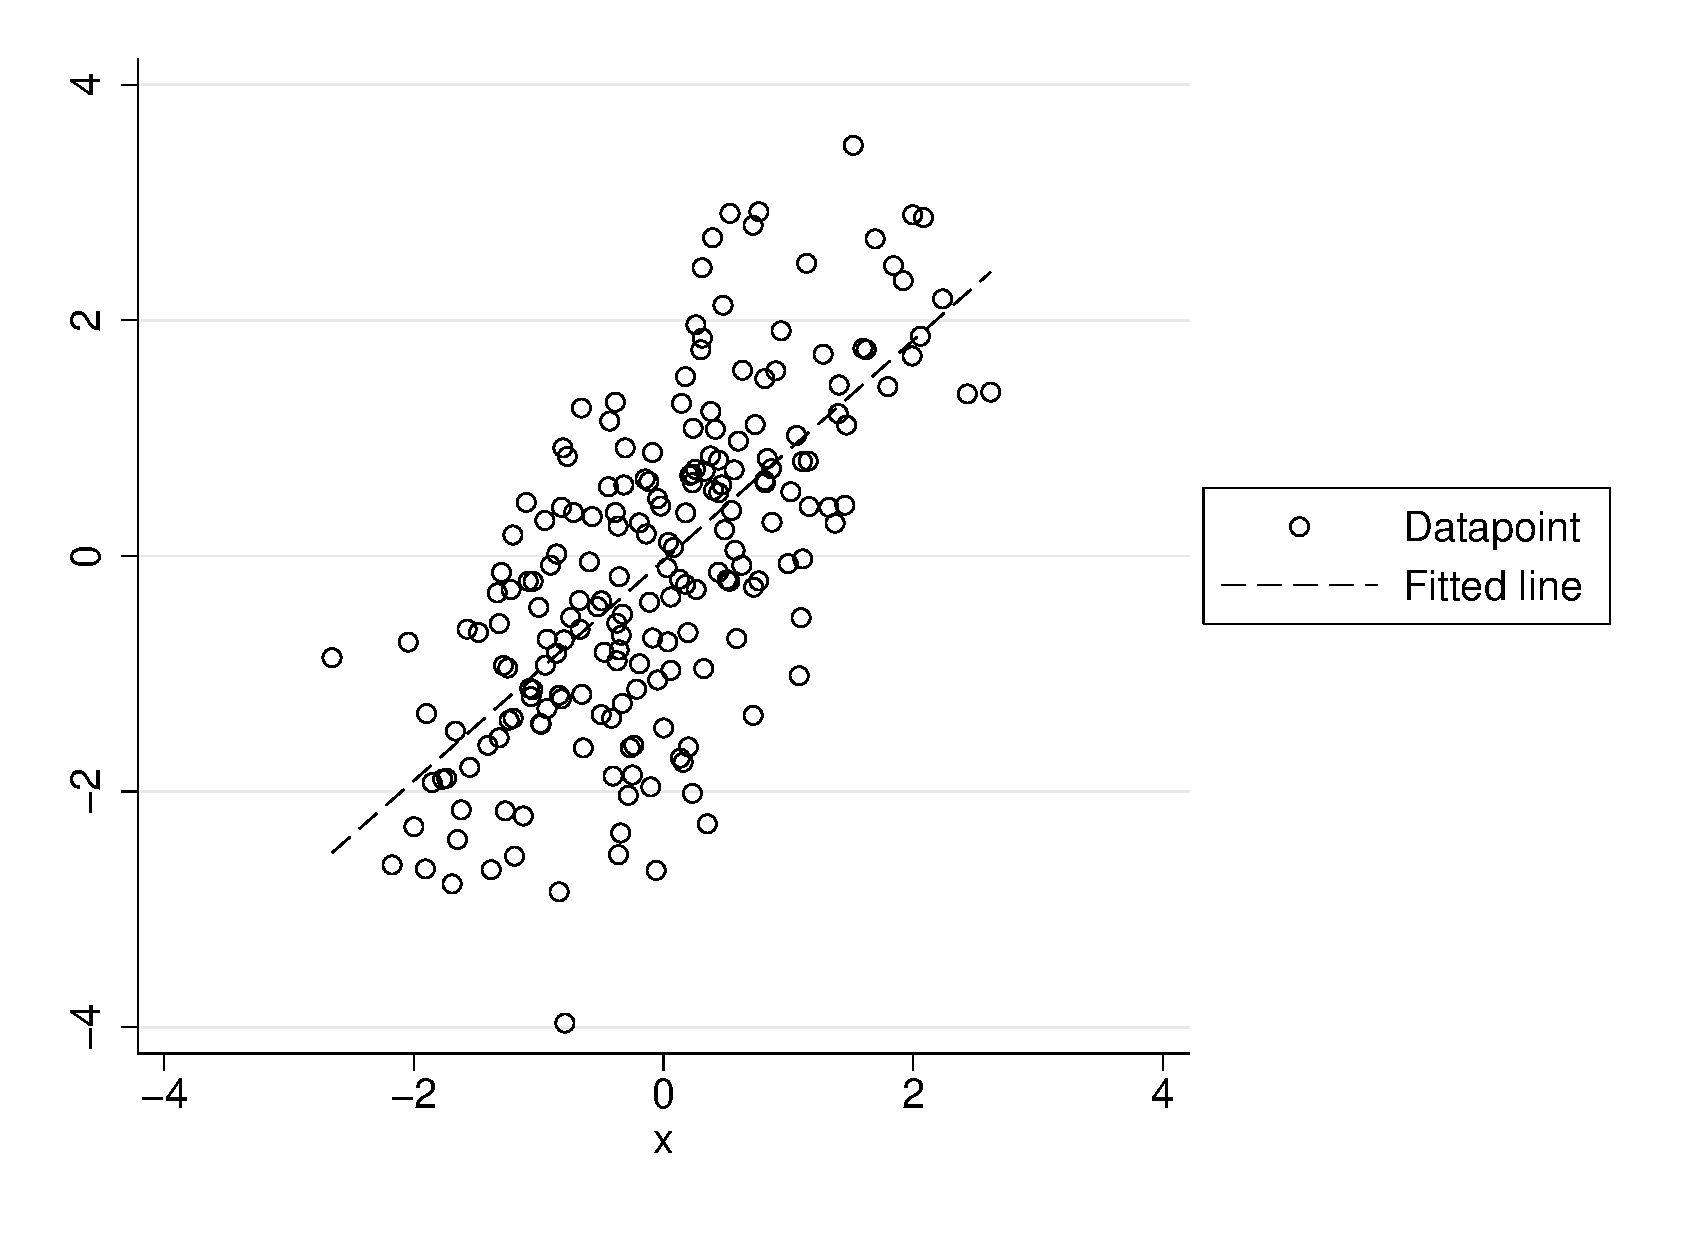
\includegraphics[angle=0,
           width=.75\textwidth]{linearok.eps}
   \caption{Data where $y$ is a linear function of $x$}
  \label{fig:linearok}
\end{figure}
In many cases relationships are not linear and if you do not transform the data the estimated relationships are not valid. A classic violation of this is a quadratic relationship.
\begin{figure}
   \centering
   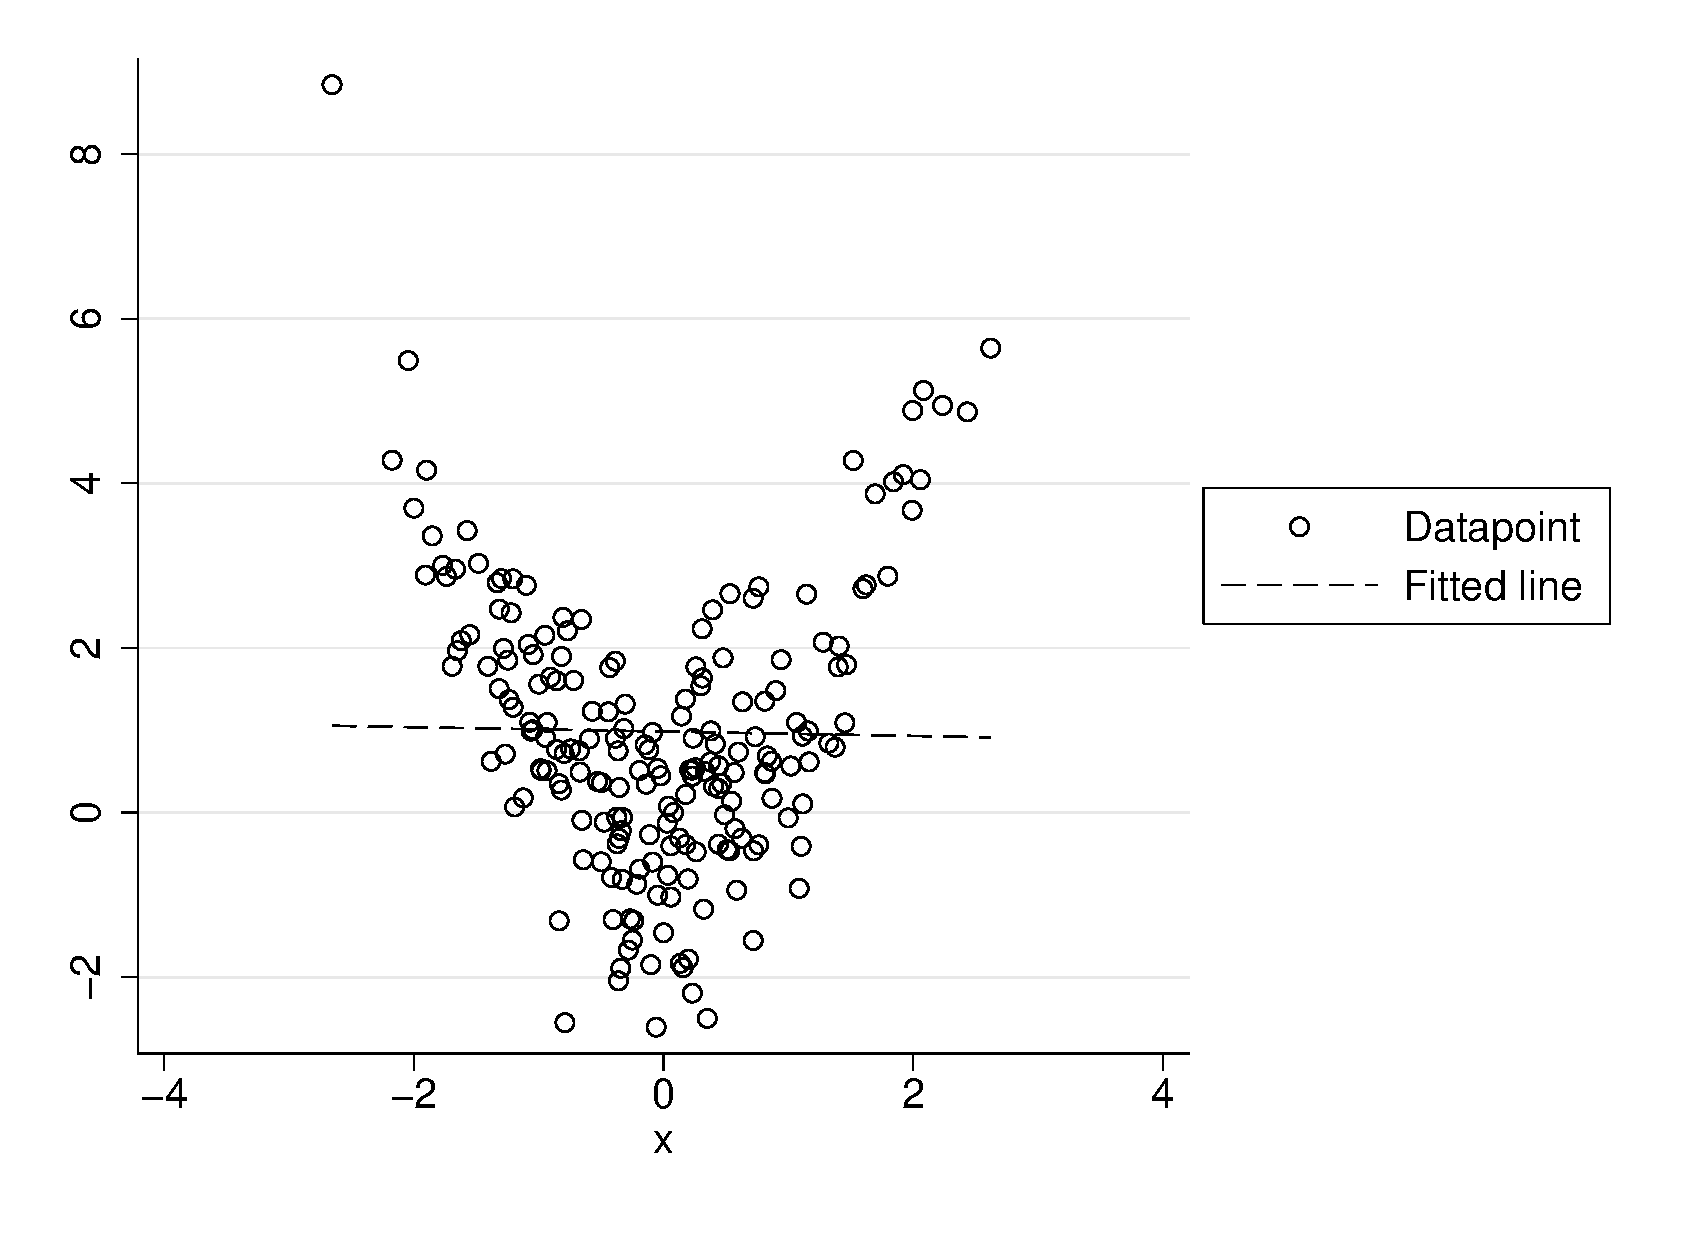
\includegraphics[angle=0,
           width=.75\textwidth]{linearnotok.eps}
   \caption{Data where $y$ is not a linear function of $x$}
  \label{fig:linearnotok}
\end{figure}
Figure~\ref{fig:linearnotok} displays this situation. When the relationship is quadratic and you fit a linear model without transformations, the slope may not reflect the data. In this case, the fitted slope is close to 0 even though it is obvious there is a relationship in the data.
Unfortunately, there is no easy way to check this assumption outside of a examining the data. This is why we have theory. The best regression diagnostic is theory. Your model should be governed by theory. Trust your theory.
\subsection{The expected value of any residual is zero}
Related to the previous assumption is that we assume that the expected value of a residual is 0. "Expected" is fancy statistics language for "average." Thus, we expect that the residuals to be 0, on average, for any level of predictor. The math forces this to be true overall. However, I find more nuanced way of thinking of this assumption is to assume that for every value of x, the expected value of the residuals is 0. If we have a multivariate model, then instead of x we can use the fitted value of y.
\begin{figure}
   \centering
   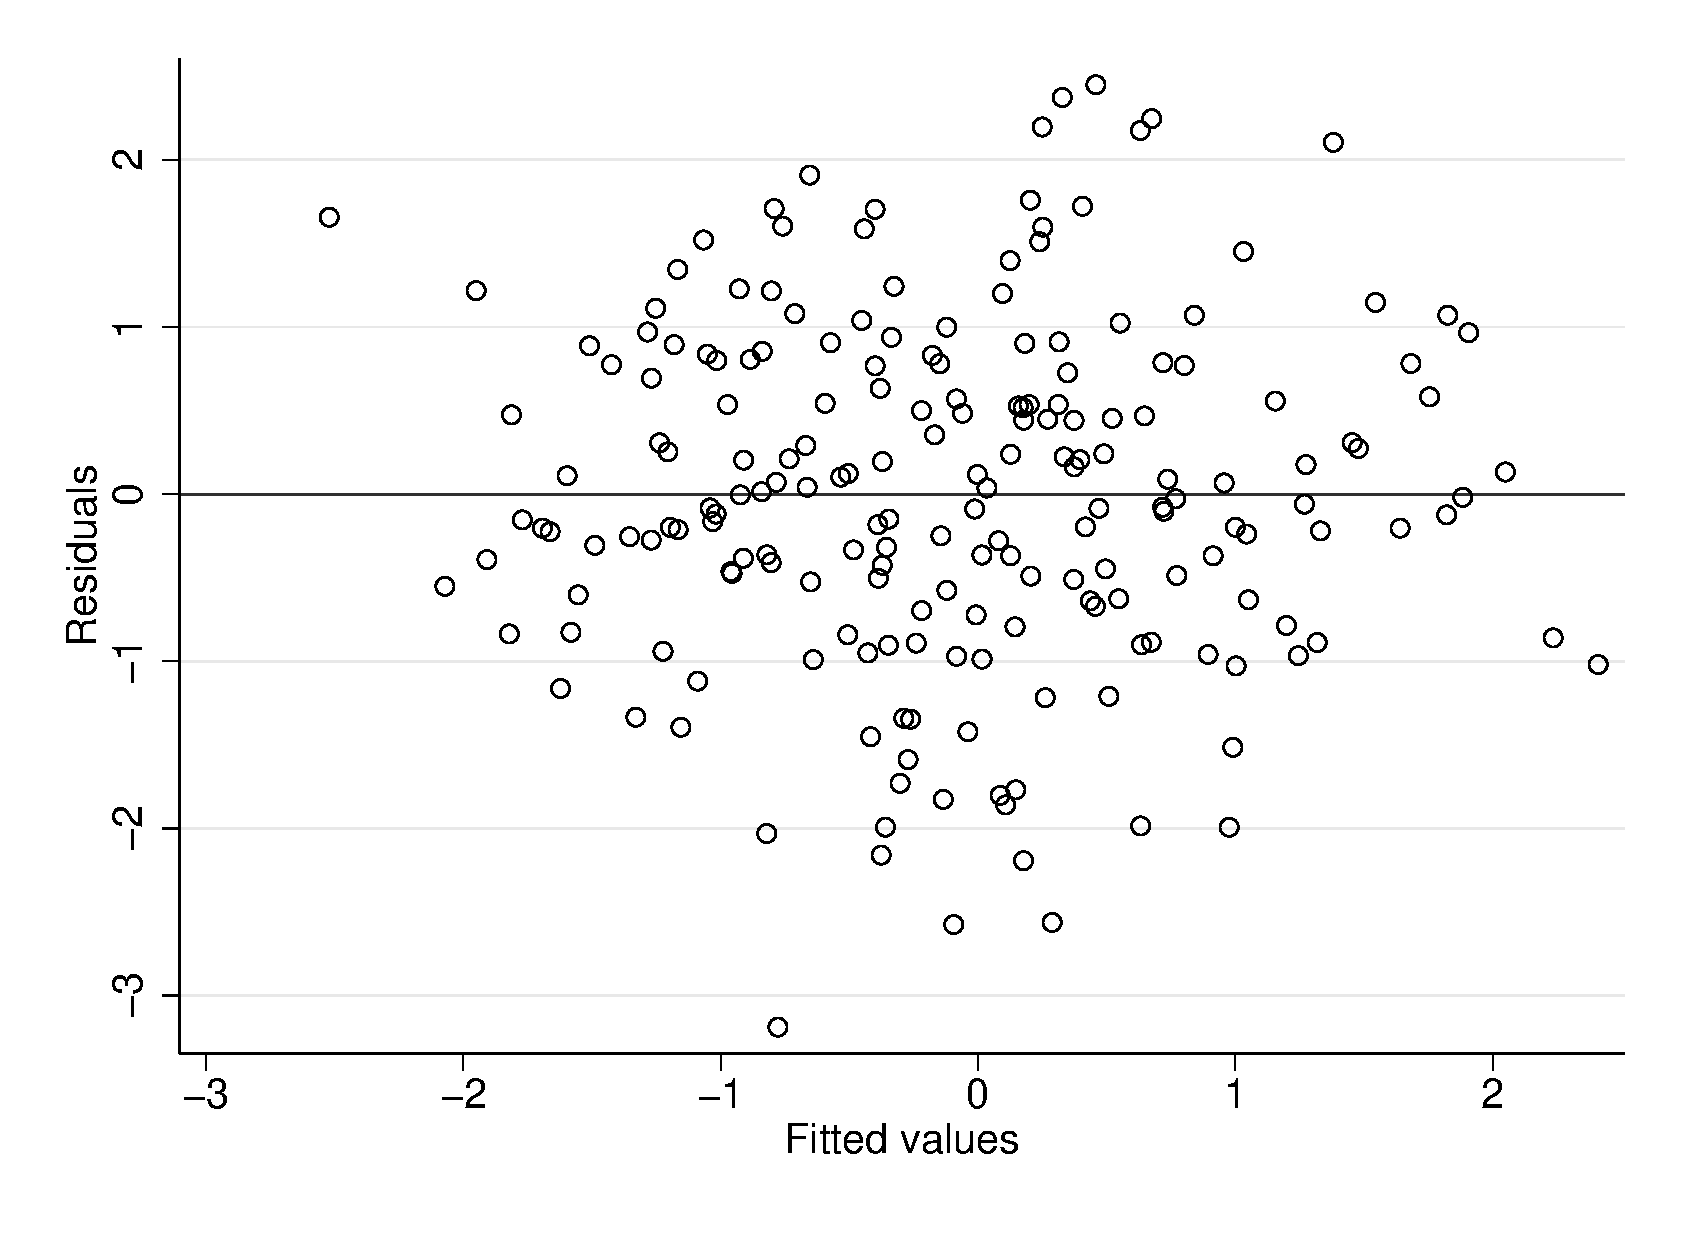
\includegraphics[angle=0,
           width=.75\textwidth]{mean0ok.eps}
   \caption{Data where $e$ is zero on average}
  \label{fig:mean0ok}
\end{figure}
The reason we can use a fitted value of y is that the fitted value of y is just a linear combination of all the predictors. We can inspect this visually by making a scatterplot of the residuals by the fitted values, see Figure~\ref{fig:mean0ok} where we meet the assumption that residuals average to 0. If, on the other hand, there is some pattern to the residuals, like in a un-modeled quadratic relationship, the plot may look like Figure~\ref{fig:mean0notok}.
\begin{figure}
   \centering
   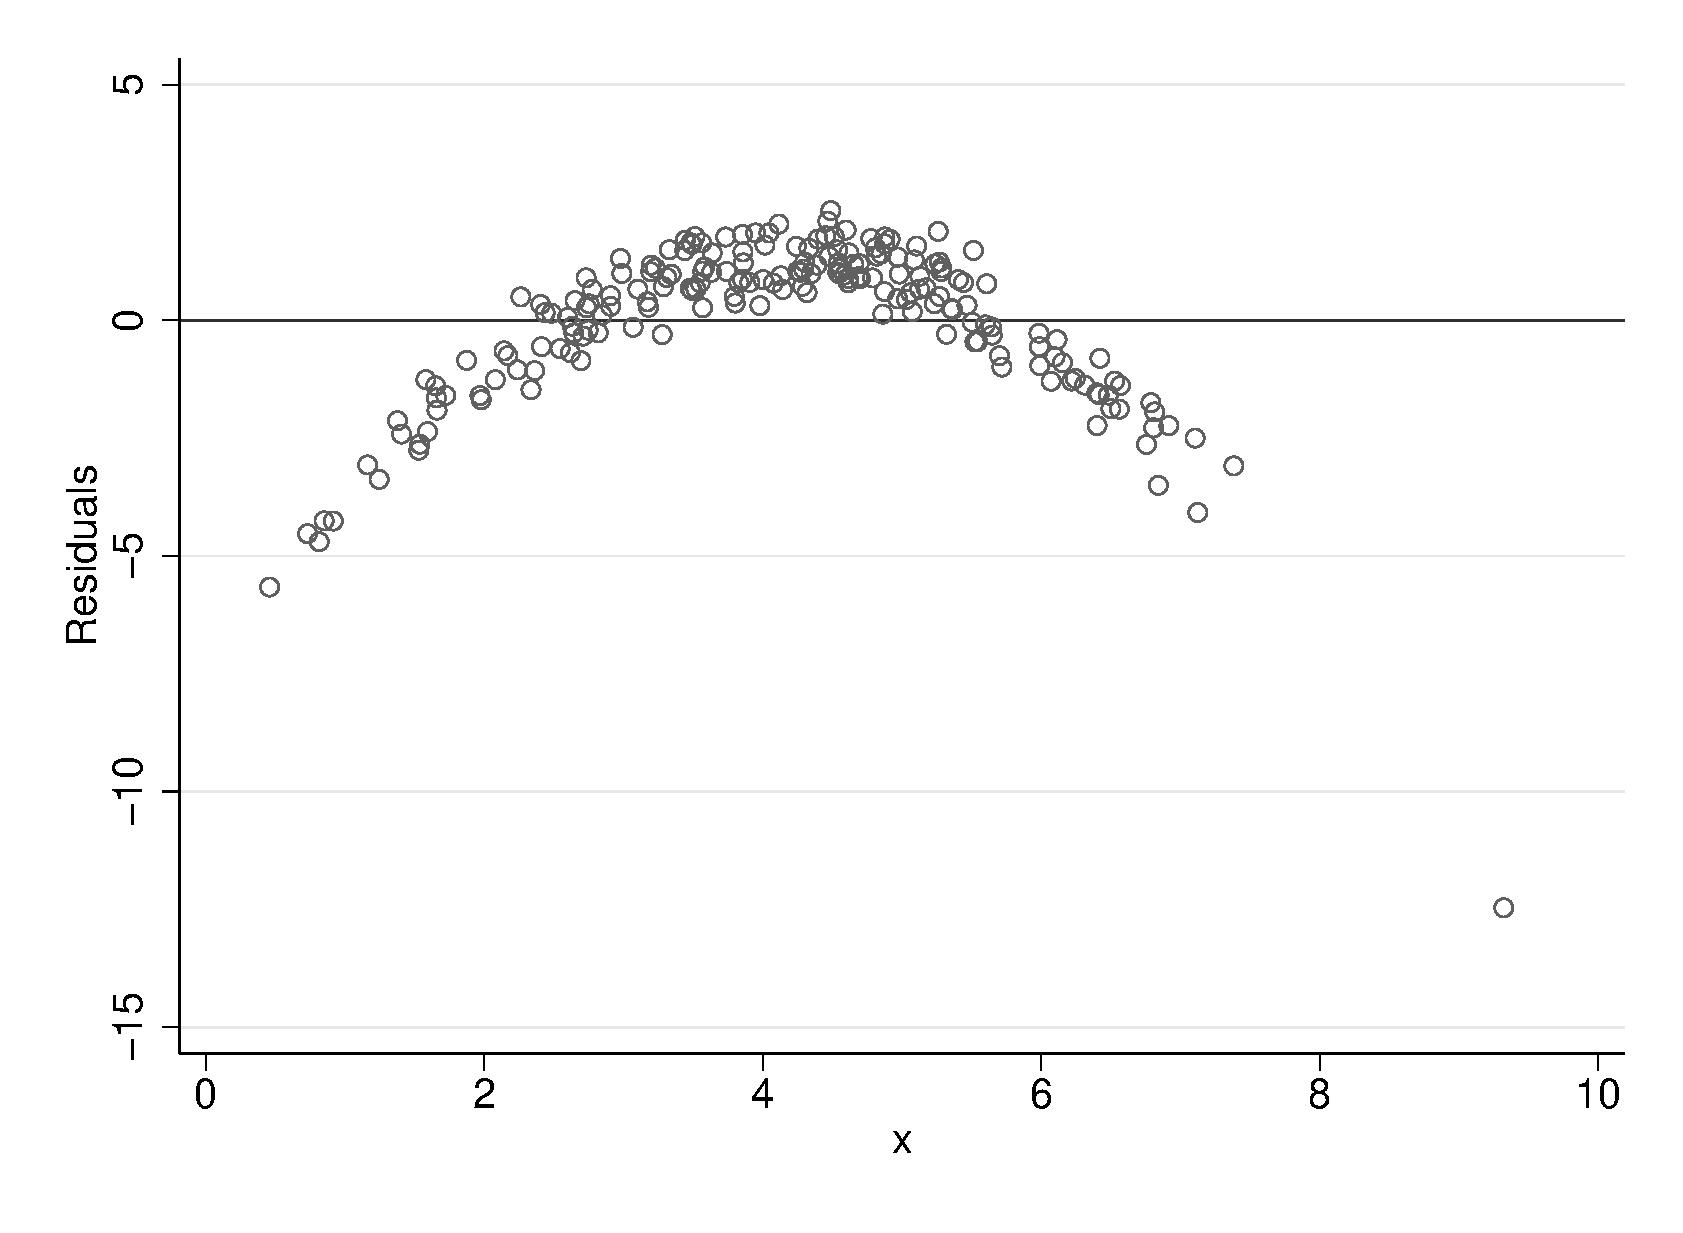
\includegraphics[angle=0,
           width=.75\textwidth]{mean0notok.eps}
   \caption{Data where $e$ is not zero on average}
  \label{fig:mean0notok}
\end{figure}
\subsection{The variance of the residuals is constant}
As we will see throughout the book, many of the formulas for standard errors and other measures make the assumption that there is a single variance for all the residuals, $\sigma^2$.

However, in many situations this is not the case. When this assumption is violated, standard error become biased, making hypothesis tests difficult. Often this happens for practical reasons. For example, we will look at an example where charitable giving is a function of income. When income is low, there is little variance in giving because those who do not have a lot of money cannot give anything. At the other end, there is quite a bit of variance: you have people like Bill Gates who give a lot, and people like Steve Jobs who did not give much (at least publicly). When this is violated, you may see a "fan" pattern in your residuals like in Figure~\ref{fig:hetero}
\begin{figure}
   \centering
   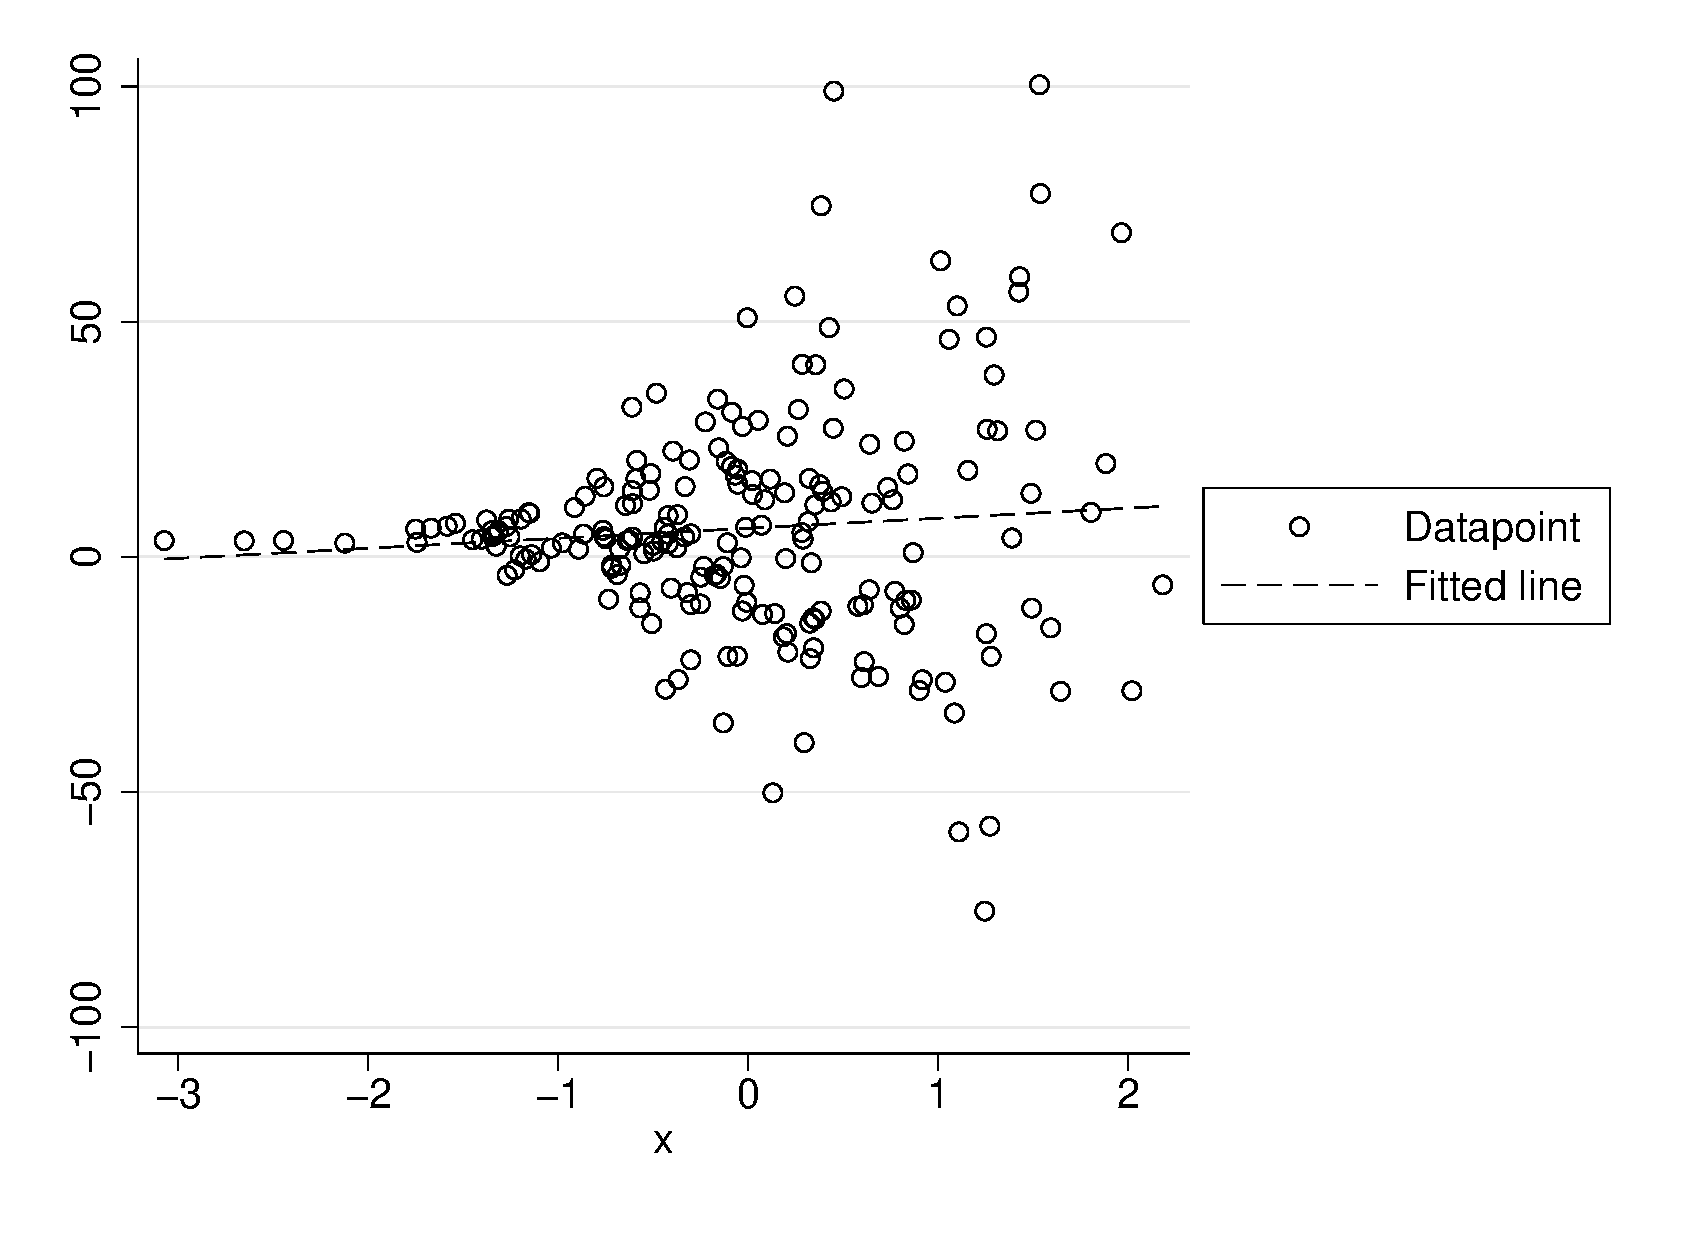
\includegraphics[angle=0,
           width=.75\textwidth]{hetero.eps}
   \caption{Data where $e$ does not have constant variance}
  \label{fig:hetero}
\end{figure}
\subsection{The covariance of all residuals is zero}
One of the most commonly violated assumptions is that all the residuals are independent. We can express this as
\begin{equation}
\mbox{cov}\left(e_i,e_j\right)=0
\end{equation}
There are several ways in which observations of y can be correlated:
\begin{enumerate}
 \item Observations are adjacent to each other across time
 \item Observations are members of common geographical regions
 \item Observations are members of other common meaningful clusters
 \item Any combination of the above, and more
\end{enumerate}
This is an old problem in social science and survey research. There are many solutions to this issue and we cover many of them in these notes.
\subsection{The values of the predictors are not random}
In normal regression we assume that the predictors, especially the intercept, are not random variables.  When we cluster sample, that is sample groups then units within those groups, the intercept can be argued to be a random variable and thus violating this assumption.  Another example is time within units.  Many of the multilevel models are designed to compensate for this issue.
\subsection{The values of the predictors are not exact linear combinations of each other}
This assumption is pretty easy to confirm. If it is violated, and one variable is exactly correlated with another, it is impossible in invert . Many software packages with automatically remove offending variables from models.
\subsection{The errors are distributed normally}
Many students misunderstand this assumption to mean that the outcome needs to be distributed normally. This is not the case. The residuals, the outcome net of the model, must be normally distributed.
For example, consider a model a continuous predictor $x$ and another dichotomous predictor $z$. A histogram of the data appears in Figure~\ref{fig:dummyhist} and you can see the bi-modal distribution. We see in Figure~\ref{fig:dummyhist_r} that net of the model the errors are almost normally distributed. We need to make this assumption to prove that the least squares estimator is the maximum likelihood estimator.
\begin{figure}
   \centering
   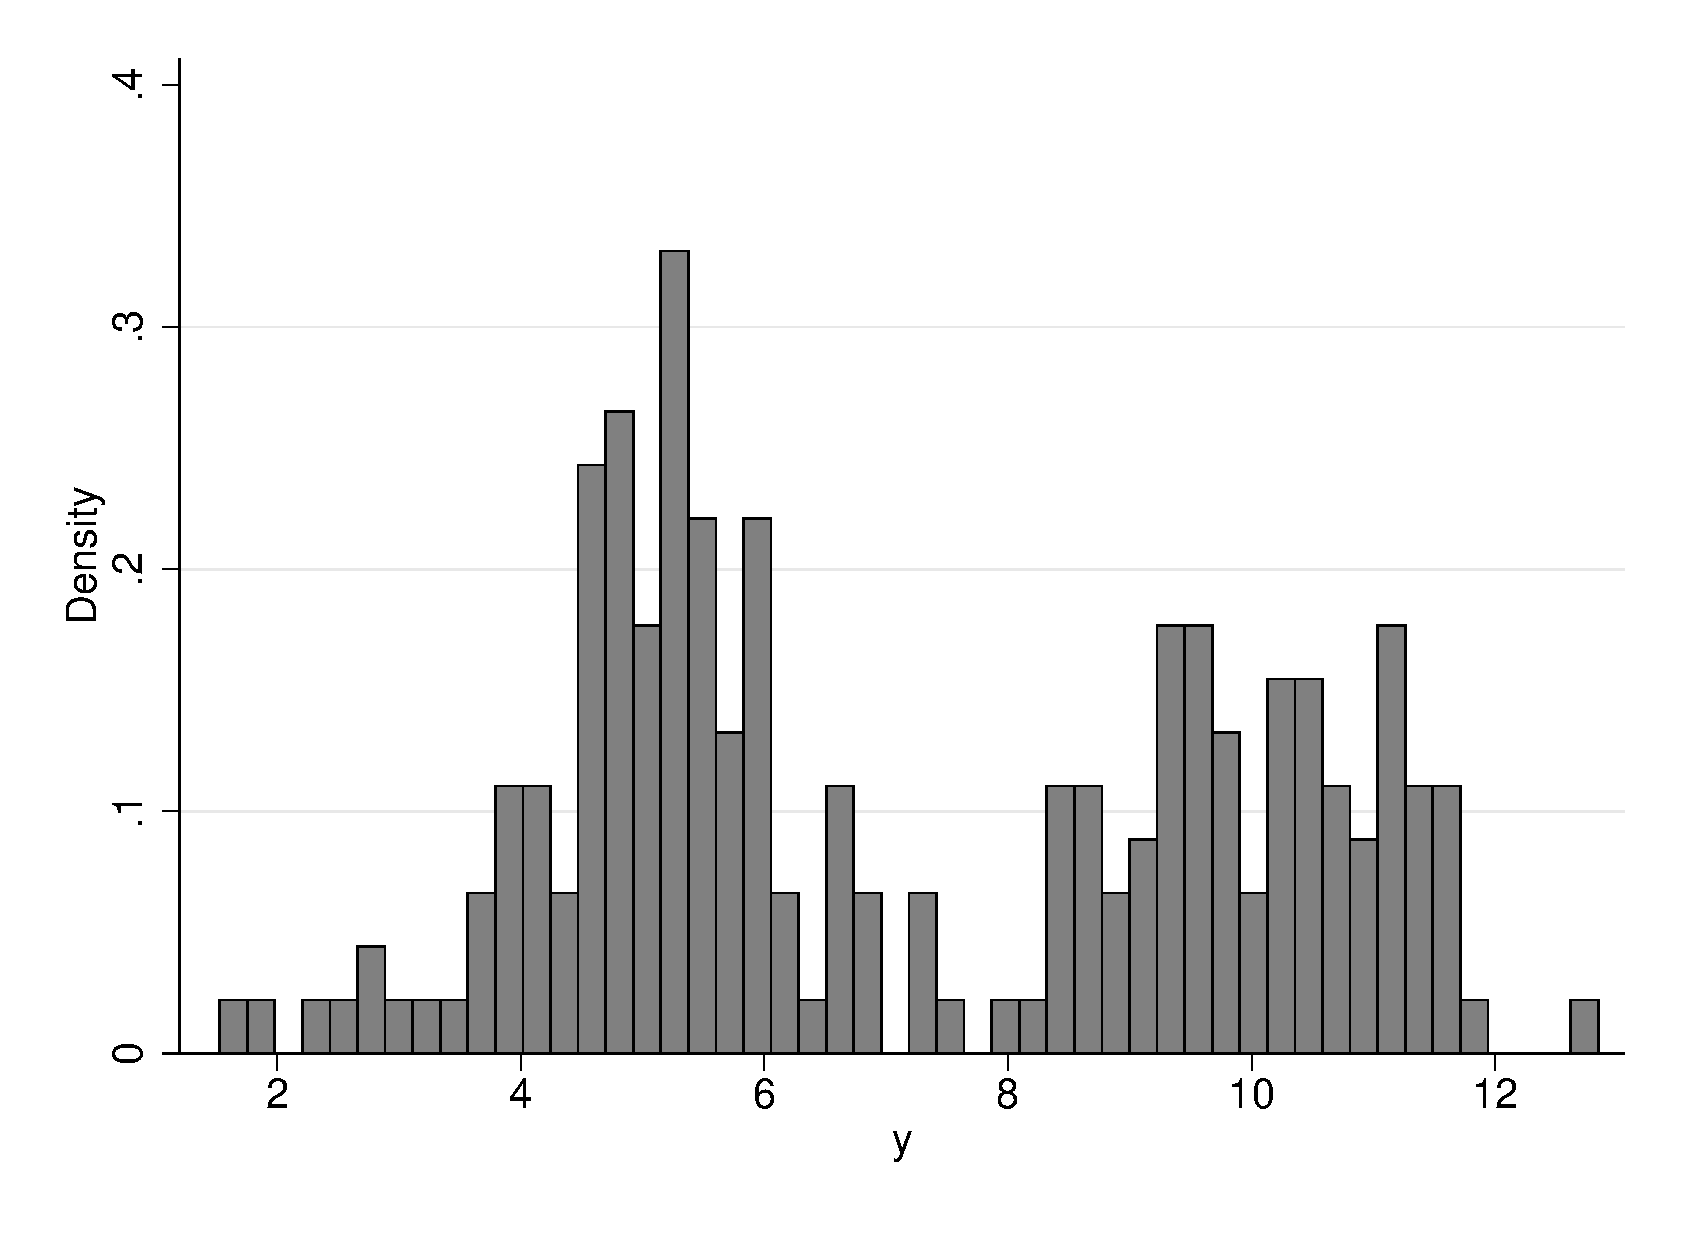
\includegraphics[angle=0,
           width=.75\textwidth]{dummyhist.eps}
   \caption{Data $y$ as a function of a dummy variable}
  \label{fig:dummyhist}
\end{figure}
\begin{figure}
   \centering
   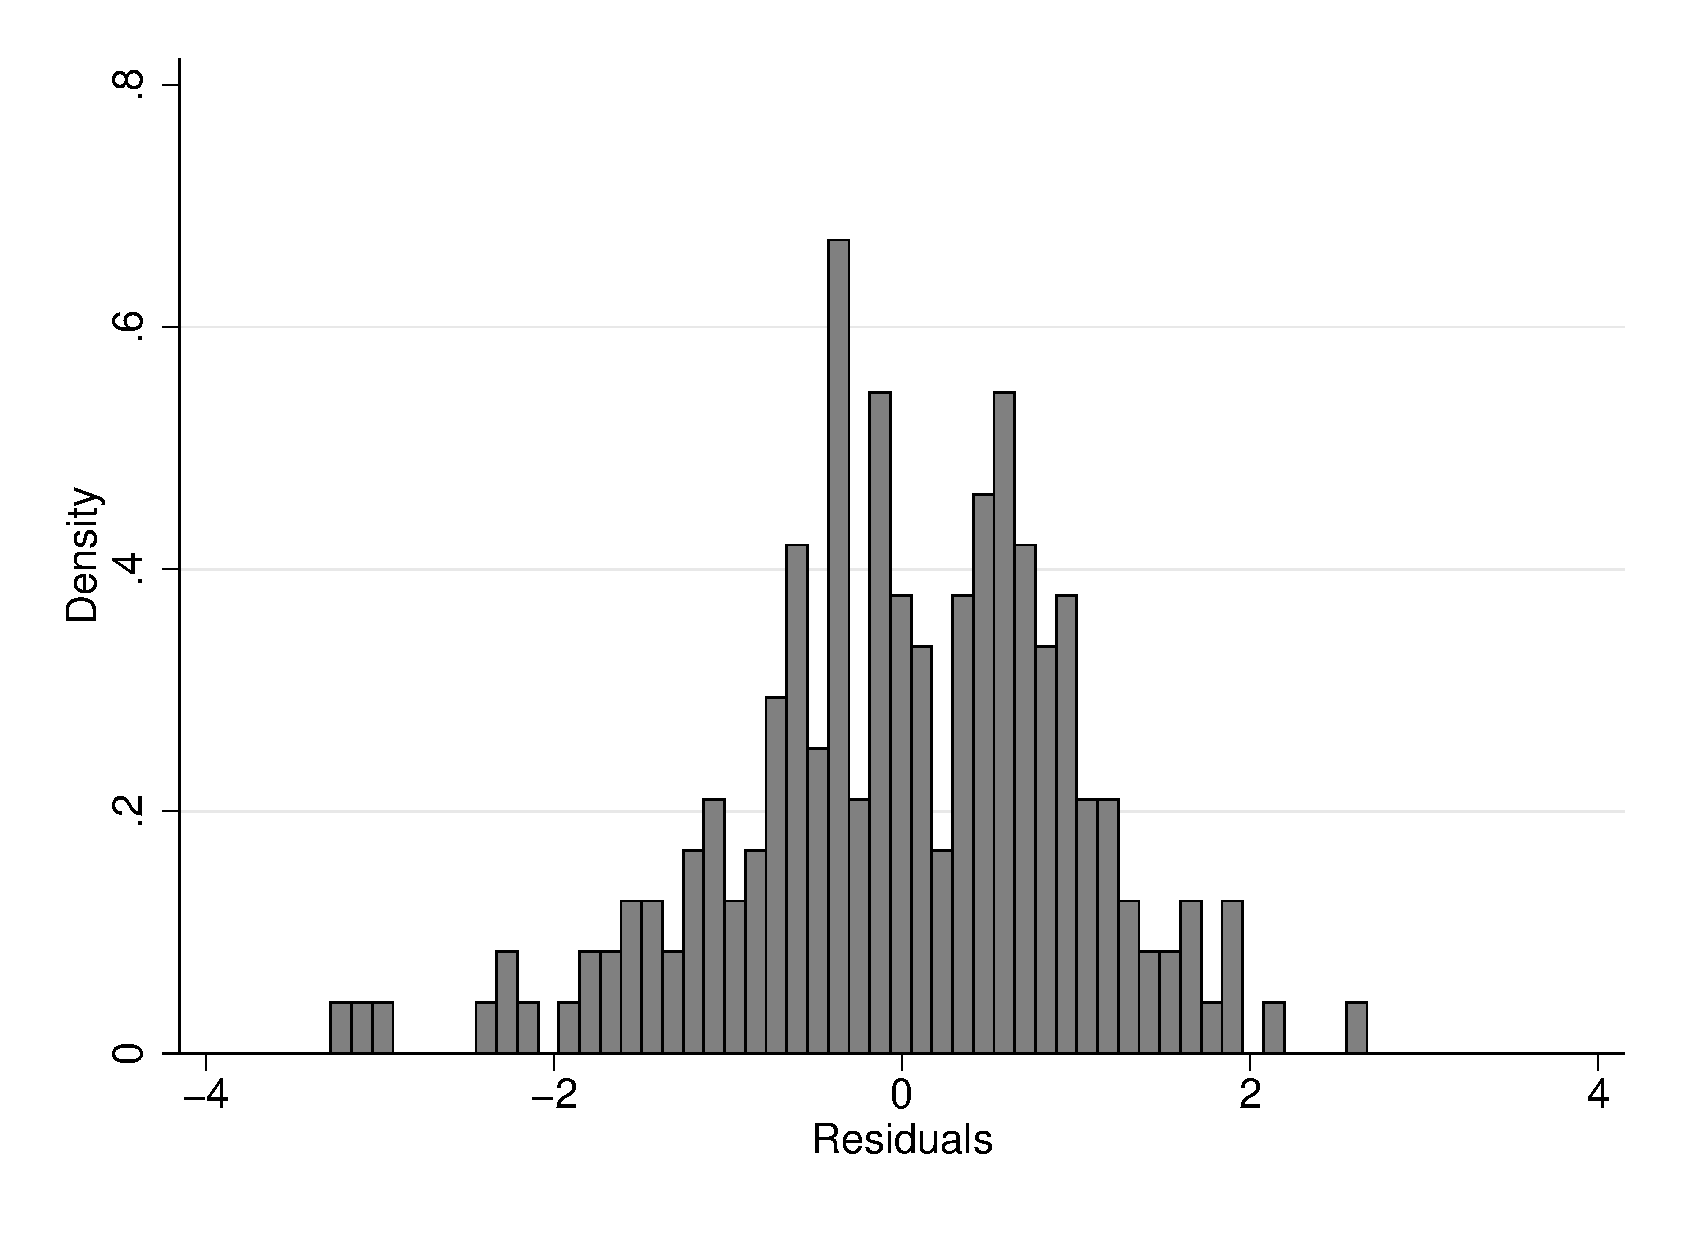
\includegraphics[angle=0,
           width=.75\textwidth]{dummyhist_r.eps}
   \caption{Residuals of a model for $y$ that included a dummy variable}
  \label{fig:dummyhist_r}
\end{figure}

However, sometimes there is no way to achieve normal errors. Situations in which the outcome is dichotomous or a count variable with a large proportion of zeros will never produce normally distributed outcomes. In those situations we need to use generalized linear models (GLMs). 